\documentclass[a4paper,showframe,11pt]{report}
\usepackage{standalone}
\standalonetrue
\ifstandalone
  \usepackage{../../haziq_thesis}  
  \usepackage{../../haziq_maths}
  \usepackage{../../haziq_glossary}
  \usepackage{../../knitr}
  \addbibresource{../../bib/haziq.bib}
  \externaldocument{../01/.texpadtmp/chapter1}
  \externaldocument{../02/.texpadtmp/chapter2}
  \externaldocument{../03/.texpadtmp/chapter3}
  \externaldocument{../04/.texpadtmp/chapter4}
  \externaldocument{../05/.texpadtmp/chapter5}
\fi

\begin{document}
\hChapterStandalone[6]{Bayesian variable selection using I-priors}
\label{chapter6}

Earlier in \cref{chapter4}, \cref{sec:various-regression}, we saw that model \cref{eq:model1} subject to normal assumptions \cref{eq:model1ass}, model assumptions \ref{ass:A1}--\ref{ass:A3}, and $f$ belonging to the canonical RKHS of functions over $\cX \equiv \bbR^p$ yields the standard multilevel regression model
\begin{align}\label{eq:linmod}
  \begin{gathered}
    y_i = \alpha + \sum_{k=1}^p x_{ik}\beta_k + \epsilon_i \\
    \epsilon_i \iid \N_n(0, \sigma^2).
  \end{gathered}  
\end{align}
In this chapter, we use the notation $\sigma^2 = \psi^{-1}$ to denote the error variance.
Furthermore, an I-prior on the regression coefficient entails prescribing the following normal prior the $\beta_k$'s:
\[
  \bbeta := (\beta_1,\dots,\beta_p)^\top \sim \N (\bzero, \sigma^2 \kappa \XTX).
\]
This follows from \cref{eq:ipriorcanonical} after a slight reparameterisation of the RKHS scale parameter $\kappa \mapsto \lambda^2/\sigma^4$. 
Throughout this chapter, we assume that the columns of the design matrix $\bX = (X_1,\dots,X_p)$ have been standardised, so that a single RKHS scale parameter is sufficient for the $p$ covariates.

The topic of interest for this chapter is variable selection, or more generally, model selection.
Model selection entails searching the entire model space to find the ``best'' model according to some criterion. 
There are many such criteria, from both frequentist and Bayesian perspectives, making model selection a huge topic to cover fully. 
These include the (adjusted) $R^2$, Akaike's information criterion (AIC), Bayesian information criterion (BIC) and other similar information criteria, Mallow's $C_p$, ($k$-fold) cross-validation error, and so on. 
Methods such as forward or backward selection provide heuristic approaches to model selection, but never truly explore the entire model space.

On the other hand, regularised least squares regression (ridge regression, Lasso, elastic nets, etc.) provides additional information to the linear model in order to provide a sparse solution to linear system of equations in $\bbeta$.
These methods are proven to be popular and work well even in cases where $p > n$.
From a Bayesian perspective, this is akin to placing priors on the $\beta_k$'s to shrink the effects of the $\beta_k$'s.
Regularisation is fine when the ultimate goal is to `cut down the number of variables' or to obtain a particular quantity of interest, such as prediction.
However, often times there is a genuine desire to know the most reasonable, parsimonious and interpretable model---a goal which is achieved through model selection.
Through variable selection, we learn which covariates are important, and which are negligible.

There is a massive literature concerning Bayesian variable selection \citep{Chipman2001,OHara2009}.
The approach that we take is a stochastic search of the model space due to \citet{George1993,Kuo1998} realised through a simple Gibbs sampling procedure.
The plan for this chapter is to describe a fully Bayesian stochastic approach for variable selection using I-priors. 
%A Gibbs sampling procedure is used to obtain posterior estimates of model probabilities.
The main motivation behind using I-priors in Bayesian variable selection is its suitability in accommodating to datasets with strong multicollinearity and being able to run with little to no prior information about the parameters.
A simulation study is conducted and several real-world examples presented to demonstrate this fact. 

%The obvious issue is that when the dimension of the model space is large, then a search of the entire model space may be computationally prohibitive or even downright unfeasible. 

%The general framework behind model evaluation may be thought of as follows: it is believed that a dataset $\by = (y_1,\dots,y_n)$ had been generated from the pdf $f(y|M_k, \Theta_k)$, where $M_k$ is one of many possible models\footnote{We refer to these as models not in the usual sense - more precisely, each $M_k$ is a model class.}~from the set $\cM=\{M_1, \dots, M_K\}$, where $\Theta_k$ are the parameters associated with this model. 
%The goal of model selection is then to infer which of the $K$ models had generated the data, and consequently obtain estimates for $\Theta_k$. 
%The Bayesian approach allows us to assign priors to the parameters and the model index, i.e. $p(\Theta_k|M_k)$ and $p(M_k)$ respectively, such that \emph{posterior model probabilities} may be calculated as
%\begin{align}\label{eq:pmp}
%	p(M_k|\mathbf y)	&\propto p(y|M_k)p(M_k) \nonumber \\
%	&\propto \int p(y|M_k, \Theta_k)
%	p(\Theta_k|M_k) \dint\Theta_k \, p(M_k).
%\end{align}
%The natural criteria for choosing $M_k$ is one that gives the highest posterior probability. 
%We refer to this model as the highest probability model (HPM). 

%Our problem may be simple enough that we are able to calculate all of the posterior probabilities, in which case the task is as simple as reading off the HPM from a list of models with their corresponding probabilities. 
%However, this is likely not the case, and we often have a large model set to consider. 
%Even if the model set is small, we might find that the integral in the posterior is not analytically tractable. 
%In either of these cases, Markov chain Monte Carlo (MCMC) methods is suitable to be used to overcome these issues of calculating the required posterior probabilities. 
%In fact, MCMC methods can be quite efficient in the exploration of the model space because it  will favour models which have great potential of being the true model, and will tend to ignore those that have little to no potential. 

%While the description we have just given for model selection is a generic one applicable to most statistical models, variable selection is a special case of model selection to where the model at hand is defined by the inclusion or exclusion of a finite number of variables.
%The linear regression model \cref{eq:linmod} is such an example. 

\newpage
new plan: variable selection via three methods: 1) model comparison via some criterion (frequentist and Bayes); 2) shrinkage to induce sparsity; 3) Bayesian model selection (probabilities on models).

problem: on linear regression models, choice of which subset of variables should be included in the model.
explaining response variable with large number of explanatory variables.
select a small subset, as close as possible to the true generative data process, which explains most of the variation in the response.
belief of sparseness, that not all variables need to be included.

1) model selection criteria. methods described in \citep{miller2002subset}. broadly three types: prediction criteria (R2, MSEP, Mallow's Cp, CV), likelihood/information criteria (AIC,BIC). requires comparison of all $2^p$, so usually use stepwise procedures: forward-selection, backward-selection, etc. these are `heuristic methods to restrict attention to a smaller number of potential subsets' \citep{George1993}. as a rough rule, possible if predictors are less than 25 (order $10^7$).

2) shrinkage. induce sparseness by adding a penalty term to the likelihood in ML estimation (Ridge regression, Lasso, elastic net, etc.). idea is to add additional information to the system to regularise it. pros and cons?

Bayesian point of view is just to add priors.  term adaptive shrinkage has been thrown around, to give suitable shape to the prior: if important, then flat, if useful then sharp peak. requires tuning, affects mixing in MCMC chain \citep{OHara2009}. jeffreys' prior (no tuning), exponential prior (Bayesian Lasso \citep{park2008bayesian}).


3) bayesian model selection. probabilistic approach to model selection: put priors on model space, then estimate posterior model probabilities from data. slightly related to likelihood based criterion of model selection (post. model prob = BF calculations = marginal likelihoods), so if $2^p$ is large then difficult. however, the advantage of bayesian framework is the ability to apply MCMC as a practical means of overcoming the intractability. stochastic approach to model selection were pioneered by \citep{George1993}, and revisited by others \citep{Kuo1998,dellaportas2002bayesian,Ntzoufras2008}

advantages: bayesian model averaging. useful when several competing models have high posterior probabilities.

criticisms: The topic of subset selection in regression is one that is viewed by many statisticians as ‘unclean’ or ‘distasteful’. Terms such as ‘fishing expeditions’, ‘torturing the data until they confess’, ‘data mining’, and others are used as descriptions of these practices. \citep{miller2002subset}
in many studies variables are chosen because there is an expectation that they influence the response, and therefore regression model fitted is used to infer the strength of the influence.
variable selection as an exploratory study. justified by many practical applications.
arguably variable selection from a prescreening as part of data cleanup to remove problematic variables, such as those inducing a high degree of collinearity. how do we know we are deleting the correct variable?

In addition to model selection, any quantity of interest, say regression coefficients, predicted values, and any others, may be obtained by way of Bayesian model averaging.
Instead of conditioning on a single selected model, a quantity of interest $\Delta$ is averaged over a set of models to avoid underestimation of the uncertainty surrounding it \citep{madigan1994model}.
In essence, the posterior distribution of $\Delta$ may be found by averaging the model specific posterior distributions weighted by its posterior model probabilities
\begin{align}\label{eq:bma}
  p(\Delta|y) = \sum_{k=1}^K p(\Delta|y,M_k)p(M_k|y).
\end{align}
Technically, the sum should be taken over the set of all possible models, but in practice this might not be achievable.
Regardless, even if a smaller subset of models is used, it is well known that predictive accuracy of $\Delta$ is improved, as measured by a logarithmic scoring rule \citep{raftery1997bayesian}.






























\newpage
\section{Motivation: model selection and a stochastic approach}\label{sec:bvs-iprior}

The paradigm of model selection is as follows. 
From a finite set of models $\cM = \{M_1,\dots,M_K\}$, pairs of data $\{(y_1,\bx_1),\dots,(y_n,\bx_n)\}$, $y_i\in\bbR$ and $\bx_i\in\cX\equiv\bbR^p$, had been generated according to the generative process dictated by one of the models $M_k \in \cM$ and its respective parameters $\Theta_k$.
Having observed only this data set, the goal is to infer which of the models had generated the data, and consequently obtain estimates for the parameters.
%One would be inclined to evaluate and compare models by means of a criterion of some kind, and indeed many have been suggested in the literature.
It is perhaps most natural to ponder which of the models is most likely to be the ``true'' one given the data presented, and thus this natural way of thinking leads one to the concept of \emph{model probabilities}.
From a Bayesian perspective in particular, \emph{posterior model probabilities} allow us to quantify the certainty to which any model is behind the data generative process, after taking into account relevant evidence (observation of the data).

Let $\Prob$ be a probability distribution over the model space $\cM$, and denote the probability distribution function by $p(\cdot)$.
Posterior model probabilities may then be evaluated as follows. 
For any model $M_k \in \cM$, the posterior model probability for model $m$ is
\begin{align}\label{eq:pmp}
  \Prob(M=M_k|\by) &\propto p(\by|M_k)p(M_k) \nonumber \\
  &\propto \int p(\by|M_k,\Theta_k)p(\Theta_k|M_k) \dint\Theta_k \, p(M_k).
\end{align}
As a remark, the prior distributions for the parameters do not necessarily need to depend on the model, so we might have that $p(\Theta_k|M_k)=p(\Theta_k)$.
Also, the normalising constant in \cref{eq:pmp} is of course the marginal distribution for $\by$, and is found by summing \cref{eq:pmp} over all possible models, i.e.
\begin{align}\label{eq:normconst}
  p(\by) = \sum_{k=1}^K \bigg\{ p(M_k) \int p(\by|M_k,\Theta_k)p(\Theta_k|M_k) \dint\Theta_k \bigg\}.
\end{align}

The integral found in \cref{eq:pmp} and \cref{eq:normconst} is known as \emph{model evidence}.
As the name suggests, it quantifies the amount of support for a particular model being the true model.
It can also be viewed as the marginal likelihood under model $M_k$, so we denote it by $p(\by|M_k)$.

Model selection based on posterior model probabilities can be formalised as the Bayesian alternative to classical hypothesis testing using Bayes factors \citep{kass1995bayes}.
The Bayes factor for comparing any model $M_k \in \cM$ to a base model $M_0$ is given by
\[
  \text{BF}(M_k,M_0) = \frac{p(\by|M_k)}{p(\by|M_0)}.
\]
With a little manipulation, the posterior model probabilities can be calculated in terms of Bayes factors with respect to a base model.
Also, the Bayes factor for comparing any two models $M_k,M_{k'} \in \cM$ can also be calculated in terms of Bayes factors with respect to a base model:
\[
    \text{BF}(M_k,M_{k'}) = \frac{\text{BF}(M_k,M_0)}{\text{BF}(M_{k'},M_0)}.
\]

There are two potential issues with model comparison using posterior model probabilities or Bayes factors.
The first is that the calculation of the model evidence may involve an integral which might be difficult to deal with.
In the case of the linear model, this can be overcome by the use of conjugate priors for the regression model.
As an aside, one of the main reasons why $g$-priors \citep{zellner1986assessing} are very convenient to use for linear models is the fact that it completely simplifies the algebra in the posterior.

Even if all the relevant expressions can be obtained easily, there is the remaining issue that all of posterior probabilities must be calculated in order for a comparison to be made.
When the model space is very large, this can prove to be an insurmountable task.
In the case of linear regression, where each of the $p$ variables may be selected or not, the size of the model space is $2^p$.
Even for moderate sized $p$ this can already be a challenge computationally.

Markov chain Monte Carlo (MCMC) methods may be used to evaluate the posterior model probabilities.
Naturally, models which are deemed important by virtue of data evidence are sampled more often in the posterior.
In fact, models which are unpromising might never get sampled. 
MCMC methods might not list out all possible model probabilities, but it does not need to, because models which are never visited in the posterior state space are simply assigned probability zero.
In the upcoming sections, we explain the Bayesian variable selection model that we use, and also the Gibbs sampling procedure employed to obtain the posterior model probabilities.


%, because
%\[
%  -\E\left[\log \sum_{m\in\cM'} p(\Delta|y,m)p(m|y)\right] \leq - \E\big[\log p(\Delta|y,m)p(m|y)\big]
%\]
%for any $m\in\cM'$.

\section{The Bayesian variable selection model}

%Variable selection may be viewed as a special case of model evaluation, whereby a model is defined by the inclusion or exclusion of variables. 
%The linear model \eqref{eq:linmod} defined at the beginning is an example of this, and for the remainder of this paper, we will only consider models of this type. 
Considering variable selection as a special case of model selection, we shall loosely refer to a model as a subset of variables selected from the full set of variables $\{ X_1, \dots, X_p \}$. 
Note that we do not consider the intercept to be selectable. 
If this were the case, this would imply a model as having intercept equal to zero as being possible. 
For most practical modelling purposes, the intercept is almost always non-zero.

It would be useful to be able to index each of these $2^p$ possible models somehow. 
Consider the one-to-one mapping $G:\cM \to \{0,1\}^p$ as defined by $M \mapsto \gamma = (\gamma_1,\dots,\gamma_p)$, where $\gamma_j = 1$ if the variable $X_j$ is selected, and 0 otherwise, for $j=1,\dots,p$.
As an example, the full model, where all the variables are included in the model, is denoted by $\gamma = (1, \dots, 1)$, while the intercept only model is denoted by $\gamma = (0, \dots, 0)$.

Priors on the model can then be specified more concretely, for example 
\begin{equation}\label{eq:priorgamma}
  p(\gamma) = \prod_{j=1}^p \Bern(\pi_j).
\end{equation}
We may choose to set all $\pi_j = 0.5$ a priori to reflect equally likely probabilities that any model may be chosen.
Alternatively, we might have some subjective beliefs about which predictor is more likely or unlikely to be included in the model.
We may also choose to include $\pi_j$ in the estimation procedure by assigning a hyperprior on $\pi_j$ such as the Beta(1, 1) (uniform distribution), Beta(1/2, 1/2) (Jeffrey's prior), or any other suitable hyperprior.
In any case, in this thesis we consider the simplest case of setting all $\pi_j = 0.5$.

Having considered the model prior, we now think about extending the linear model to include the indicator variables $\gamma_j$.
Following \citet{Kuo1998}, the linear model in \cref{eq:linmod} is expanded to
\begin{align}\label{eq:km}
  \begin{gathered}
    y_i|\alpha,\bbeta,\gamma,\sigma^2 \iid \N \left( \alpha + \sum_{k=1}^p x_{ik}\gamma_k\beta_k \, , \, \sigma^2 \right).
  \end{gathered}  
\end{align} 
Hence, in addition to the usual model parameters, we are interested in conducting model inferences through the posterior distribution of the $\gamma$'s.
The \citeauthor{Kuo1998} model is often known as the independent sampler due to the independence of model parameters and the indicator variables.
Prior choices for the regression coefficients include an independent prior $\bbeta\sim\N_p(\bzero,c^2\bI_p)$, the $g$-prior $\bbeta\sim\N_p(\bzero,g\XTX^{-1})$, or even the I-prior.

We complete the Bayesian variable selection model with conjugate prior choices on the remaining parameters---normal for $\alpha$ and inverse gamma for the scale parameters.
Choosing the I-prior for $\bbeta$ in particular, the prior density on the model parameters is
\begin{align}
    p(\bbeta,\alpha,\sigma^2,\kappa) 
    &= p(\bbeta|\sigma^2,\kappa)p(\alpha|\sigma^2)p(\sigma^2)p(\kappa) \nonumber \\
    &\equiv \N_p(\bbeta|\bzero,\sigma^2\kappa \XTX) \cdot \N(0,\sigma^2 A) \cdot \Gamma^{-1}(\sigma^2|c_\sigma,d_\sigma) \cdot \Gamma^{-1}(\kappa|c_\kappa,d_\kappa).
\end{align}
Choices for the prior hyperparameters depend on the user's prior beliefs, but it is reasonable to set vague and uninformative hyperparameters to let the data speak as much as it can, especially in the absence of prior information. 
With this in mind, we may choose large values of $A$ (e.g. 100) and small values of the shape and scale parameters for the inverse gamma (e.g. 0.001). 
Note that as $c_\sigma,d_\sigma,c_\kappa,d_\kappa \to 0$ then we get the Jeffrey's prior for scale parameters.

The BVS model \cref{eq:km} together with the choice of Bernoulli priors on $\gamma$ and a normal prior $\N_p(\bzero,\bV_\beta)$ for $\bbeta$ can be seen a spike-and-slab prior for linear regression models; it is a combination of a point mass at zero and a normal prior \citep{mitchell1988bayesian,geweke1996variable}.
Write $\btheta = (\gamma_1\beta_1,\dots,\gamma_p\beta_p)^\top$.
Then, the prior on the model-specific regression coefficients $\btheta$ is
\[
  \btheta|\gamma \sim
  \begin{cases}
    \N_p(\bzero,\bV_\beta) & \text{w.p. } p(\gamma) \\
    0 & \text{w.p. } 1 - p(\gamma).
  \end{cases}
\]
A subtle fact of these spike-and-slab priors is that the posterior distribution for $\btheta$ will also be a combination of a point mass and a normal density (with appropriate posterior parameters).
Looking at it from this perspective, regression coefficients are assigned zero values with positive probability, and it is this subtle fact that allows covariates to be dropped from the model.
As pointed out by \citet{Kuo1998}, the form of the variable selection model allows the selection of important variables, while simultaneously shrinking the coefficients via prior information.

As a remark, the regression coefficient of interest is not $\bbeta$, but rather $\btheta = \bgamma \cdot \bbeta$, which represents the ``model averaged'' regression coefficients.
Posterior estimates surrounding $\btheta$ will have incorporated model uncertainty discussed earlier, but $\bbeta$ on the other hand, will not.
Posterior variances for $\btheta$ will typically be larger, but more ``correct'', than variances for $\bbeta$.
%In the next section, we describe the Gibbs sampling procedure to obtain posterior samples of the parameters.

\section{Gibbs sampling for the I-prior BVS model}

The Bayesian variable selection model can be estimated using Gibbs sampling, as demonstrated originally by \citet{Kuo1998}.
The Gibbs sampling procedure about to be described is adapted from their work to include an I-prior on the regression coefficients, and estimation of an intercept and the scale hyperparameter $\kappa$ for the I-prior.

Let us denote $\Theta=\{\alpha,\bbeta,\gamma,\sigma^2,\kappa\}$ to be the full set of parameters that we wish to obtain posterior samples.
Starting with suitable initial values $\Theta^{(0)}$, we then proceed to obtain further samples $\Theta^{(1)}, \dots, \Theta^{(T)}$ by sampling each parameter from the conditional posterior density of that parameter given the rest of the parameters.
A suggested set of initial values are the maximum likelihood estimates of $\Theta$, corresponding to the empirical Bayes estimate, under the full model $\gamma=(1,\dots,1)$.

Since the priors were chosen to be conjugate to the normal regression model, the Gibbs conditional densities are straightforward to obtain and familiar to those who work with Bayesian regression models.
We start with $\bbeta$: the conditional density of $\bbeta$ given $\alpha,\gamma,\sigma^2,\kappa$ is multivariate normal with mean $\tilde \bB(\by-\alpha\bone_n)$ and covariance matrix $\sigma^2\tilde \bB$, where $\tilde B = \bX_\gamma^\top \bX_\gamma + (\kappa \XTX)^{-1}$, and $\bX_\gamma = (\gamma_1X_1 \cdots \gamma_pX_p)$.
Interestingly, when $X_j$ is dropped from the model ($\gamma_j=0$), the posterior mean and variance for $j$'th component of $\bbeta$ is entirely informed by the prior \citep{Kuo1998}.
The data-driven I-prior incorporates information from the data into the prior which then informs the posterior, but this will not be the case if subjective priors or uninformative priors for $\beta$ were used instead.
In a similar manner, the conditional density for the intercept $\alpha$ is found to be $\N(\sum_{i=1}^n(y_i - \bx_i^\top\btheta) / \tilde A,\sigma^2\tilde A)$, where $\tilde A = n + A^{-1}$ and $A$ is the prior variance for $\alpha$.

The (conditional) posterior samples of $\gamma=(\gamma_1,\dots,\gamma_p)$ are obtained component-wise, and each conditional probability mass function for $\gamma_j$ is Bernoulli  with success probability $\tilde \pi_j = u_j / (u_j + v_j)$, where
\begin{align*}
  \begin{gathered}
    u_j = \pi_j \exp\left( - \frac{1}{2\sigma^2} \Vert \by - \alpha \bone_n - \bX\btheta_j^{[1]} \Vert^2 \right) \\
    \text{and} \\
    v_j = (1-\pi_j) \exp\left( - \frac{1}{2\sigma^2} \Vert \by - \alpha \bone_n - \bX\btheta_j^{[0]} \Vert^2 \right).
  \end{gathered}
\end{align*}
Here, we have used the notation $\btheta_j^{[1]}$ to indicate the vector $\btheta$ with the $j$'th component replaced by $\bbeta_j$, and $\btheta_j^{[0]}$ to indicate the vector $\btheta$ with the $j$th component replaced by 0.
Values of 1 for $\gamma$ are more likely to be sampled when the ratio $u_j / v_j$ is greater than the prior odds $\pi_j/(1-\pi_j)$.
Specifically when the prior probabilities $\pi_j$ are all set to be 0.5, then $\gamma_j$ will be more likely to be sampled as `1' if $u_j > v_j$, i.e. if the residual sum of squares (RSS) $\Vert \by - \alpha\bone_n - \bX\btheta \Vert^2$ is \emph{smaller} when the $j$th component is non-zero, compared to the RSS when the $j$'th component of $\btheta$ is zero.

We can in fact draw parallels to a Bayesian hypothesis test, with the null hypothesis being $\text{H}_0: \beta_j = 0$ and the alternative being $\text{H}_1: \beta_j \neq 0$, conditional on knowing all other values of the parameters.
Under $\text{H}_k$, $\by|\Theta \sim\N_n(\alpha \bone_n + \bX\btheta_j^{[k]}, \sigma^2\bI_n )$, $k=0,1$. 
The conditional Bayes factor comparing the model in the alternative hypothesis ($M_1$) to the model in the null hypothesis ($M_0$) is therefore
%\begin{align*}
%  \text{BF}\big(M_1,M_0|\Theta\backslash\{\beta_j\}\big) 
%  &= \frac{p\big(\by | \beta_j\neq 0,\Theta\backslash\{\beta_j\}\big)}{p\big(\by|\beta_j = 0,\Theta\backslash\{\beta_j\}\big)} \\
%  &= \frac{e^{ - \frac{1}{2\sigma^2} \Vert \by - \alpha \bone_n - \bX\btheta_j^{[1]} \Vert^2 }}{} \\
%  &= \frac{u_j}{v_j}\cdot \frac{1-\pi_j}{\pi_j}.
%\end{align*}
\begin{align*}
  \BF(M_1,M_0) 
  = \frac{u_j/\pi_j}{v_j/(1-\pi_j)} 
  = \frac{\tilde \pi_j  }{1-\tilde \pi_j} \Bigg/ \frac{\pi_j}{ 1-\pi_j }
\end{align*}
Therefore it can be seen that
%, especially in the case of $\pi_j=0.5$ for all $j=1,\dots,p$, then
the decision to include or exclude the $j$'th variable from the model relates a hypothesis test using the Bayes factor rule, and this decision is embedded in the conditional posterior probabilities $\tilde \pi_j$.
The Gibbs sampling procedure does something that can be described as ``an automated stochastic F-test for subset selection'' \citep{Kuo1998}.

Both scale parameters $\sigma^2$ and $\kappa$ follow the conditional inverse gamma distributions
\begin{align*}
  \begin{gathered}
    \sigma^2|\alpha,\beta,\gamma,\kappa \sim \Gamma^{-1}\big(n/2+c_\sigma+1, \Vert \by-\alpha\bone_n-\bX\btheta \Vert^2/2 + d_\sigma \big) \\
    \text{and} \\
    \kappa|\alpha,\beta,\gamma,\sigma^2 \sim \Gamma^{-1}\big(p/2+c_\kappa+1, \bbeta^\top(\XTX)^{-1}\bbeta/\sigma^2 + d_\kappa \big). \\
  \end{gathered}
\end{align*}
Note that the inverse gamma distribution that we specify here is defined by its shape and scale parameter, and has the density function described in \cref{def:invgam}.
Here, $c_\sigma$, $d_\sigma$, $c_\kappa$ and $d_\kappa$ are the shape and scale hyperparameters of the inverse gamma priors on $\sigma^2$ and $\kappa$.
%Since $\kappa$ is a hyperparameter to be estimated, the posterior distribution is not dependent on the likelihood of the model.
%Only the data $\bX$ enters the posterior through the covariance matrix of $\beta$.

\section{Posterior inferences}

Having obtained posterior samples $\Theta^{(t)}=\{\alpha^{(t)},\bbeta^{(t)},\gamma^{(t)},\sigma^{2(t)},\kappa^{(t)} \}$, there are two quantities of interest in relation to model inferences. 
The first is an estimate of posterior model probabilities, given by
\begin{align}\label{eq:pmp-prop}
  \widehat \Prob(\gamma = \gamma' | \by) = \frac{1}{T}\sum_{i=1}^T [\gamma^{(t)} = \gamma'],
\end{align}
where $[\cdot]$ is the Iverson bracket.
This gives an estimate of the probability of a model coded by $\gamma'$ appearing in the posterior state space of models.
The second is a quantification of the posterior inclusion for each of the $p$ variables $X_1,\dots,X_p$, known as \emph{posterior inclusion probabilities} for a variable being selected in any model.
This is given by
\begin{align}\label{eq:pip-prop}
  \widehat \Prob(\gamma_j = 1 | \by) = \frac{1}{T}\sum_{i=1}^T [\gamma_j^{(t)} = 1], \hspace{1cm} j=1,\dots,p.
\end{align}
Posterior inclusion probabilities may also be thought of as the marginals of the posterior model probabilities across each variable.

As mentioned, posterior inferences for the regression coefficient should be done on samples for $\btheta=\gamma\cdot\bbeta$ rather than $\bbeta$ itself. 
This assures that model uncertainty is accounted for in any inferential procedure surrounding the regression coefficients.
Note that, since $\btheta$ will contain values of exactly zero when predictors are dropped out of the model, the posterior density for $\btheta$ will consist of a point mass at zero combined with a normal density.

Finally, any quantity of interest $\Delta$ can be incorporated as part of the Gibbs sampling procedure.
That is, at each Gibbs iteration $t=1,\dots,T$, calculate $\Delta^{(t)}$ as a function of the parameter values at iteration $t$.
This can be done during the Gibbs sampling process, or even after the fact as part of a post-processing procedure.
Any inference on the posterior of $\Delta$ will then have incorporated the model uncertainty from a model averaging standpoint, as discussed earlier.
As an example, suppose we are interested in the predicted value at a new covariate value $\bx_\text{new} \in \bbR^p$.
For each Gibbs sample, calculate
\[
  y_\new^{(t)} = \alpha^{(t)} + \bx_\text{new}^\top (\gamma^{(t)}\cdot \bbeta^{(t)}),
\]
and obtain a point estimate $\hat y_\new^{(t)}$ using the posterior mean or mode.
The uncertainty for this estimate is contained in the standard deviation calculated from the sample $y_\new^{(1)},\dots,y_\new^{(T)}$, from which a 95\% credibility interval for this estimate can be obtained from the empirical upper and lower 0.025 cut off points.

\section{Two stage procedure}

The variable selection procedure can be made better by a ``pre-selection'' of variables to trim off unimportant variables which reduces the size of the model space being explored.
Without appealing to other external pre-selection methods, there is actually information that we could use from Bayesian variable selection models in the form of posterior inclusion probabilities.
The procedure would work as follows:

\begin{enumerate}
  \item Run the Bayesian variable selection model and obtain posterior inclusion probabilities for each variable.
  \item Discard variables with inclusion probablities less than a certain treshold, $\tau$.
  \item Re-run the Bayesian variable selection model on the set of reduced variables.
\end{enumerate}

A natural choice for $\tau$ would be 0.5, and therefore a two-stage approach to Bayesian variable selection can then be motivated as selecting the subset of variables which constitutes what is known as the \emph{median probability model}.
The median probability model is obtained by selecting all variables with a posterior inclusion probability of greater than or equal to a half.
\citet{Barbieri2004} show that the median probability model has the property of being optimally predictive under certain strict conditions. 

The notion of a two-stage approaches are not new, as many variable selection methods in the literature generally employ a pre-selection method of some kind before running their selection process proper.
This can be based on subjective preconceptions about which variables to retain, substantive theory, or even an objective pre-selection criterion.
Two-stage procedures for Bayesian variable selection models have been used in works by \citet{Fouskakis2008} and \citet{Ntzoufras2008}. 

\section{Simulation study}

In this section, we conduct a simulation study to compare the performance of different priors in the Bayesian variable selection framework described above.
The priors on beta that are compared are the I-prior, an independent prior with large prior variance (flat/uninformative prior), and the $g$-prior with $g=n$ (unit information prior, \cite{Ntzoufras2008}).
We also make a comparison the variable selection performance of the Lasso, which, from a Bayesian perspective, is similar to setting a double-exponential or Laplace priors on the regression coefficients \citep{park2008bayesian}. 
For clarity, the Lasso model employed in the simulations is of a frequentist regularisation framework as per \citet{tibshirani1996regression}, and is neither a Bayesian variable selection model as described earlier, nor a fully Bayes implementation as per \citet{park2008bayesian}.
We felt it interesting to compare the Lasso as it is widely used for variable selection of linear models.

The experiment is to select from $p=100$ variables of a $n=150$ sample size artificial dataset which has pairwise correlations between the variables. This was inspired by the studies done by \citet{George1993} and \citet{Kuo1998} in their respective papers, albeit on a larger scale (in theirs, $p=30$).
Five different scenarios were looked at. 
For each scenario, only $s$ out of 100 variables were selected to form the ``true'' model and generate the responses according to the linear model $y\sim\N(X\beta,\sigma^2 I_{100})$. 
The signal-to-noise ratio (SNR) as a percentage is defined as s\%, and the five scenarios are made up of varying SNR from high to low: 90\%, 75\%, 50\%, 25\%, and 10\%.
Variables that were included in the model had true $\beta$ coefficients equal to one.
That is, $\beta_\text{true}=(\bone_{s},\bzero_{100-s})^\top$, where $\bone_{s}$ is a row-vector of $s$ ones, and $\bzero_{100-s}$ is a row-vector of $100-s$ zeroes.
The data generation process is summarised as follows:
\begin{itemize}
	\item Draw $Z_1, \dots, Z_{100} \iid \N(0, 1)$.
	\item Draw $U \sim \N(0, 1)$.
	\item Set $X_j = Z_j + U$. This induces pairwise correlations of about 0.5.\footnotemark
	\item Draw $\by \sim \N_{150}(\bX \bbeta_{\text{true}}, \sigma^2\mathbf I_{150})$, with $\sigma=2$.
\end{itemize}

In each scenario, we are interested in obtaining the highest probability model and counting the number of false choices made in this model after a two-stage procedure of variable selection.
False choices can either be selecting variables wrongly (false inclusion) or failing to select a variable (false exclusion).
Each scenario was repeated a total of 100 times to account for variability in the data generation process, and results are summarised in \cref{tab:simres}.
The overall results are also plotted in the form a frequency polygon (see \cref{fig:simres}).

\footnotetext{$\text{Cov}(X_j, X_k) = \text{Cov}(Z_j + U, Z_k + U) = \text{Var } U = 1$, and $\text{Var}(X_j) = \text{Var}(Z_j + U) = 2$. Thus, $\text{Corr}(X_j, X_k) = \text{Cov}(X_j, X_k) / (\text{Var}(X_j)\text{Var}(X_k))^{1/2} = 1/2$.}

\begin{table}[htb]
\centering
\caption{Simulation results (proportion of false choices) for the Bayesian variable selection experiment using the I-prior, an independent prior, the $g$-prior and the Lasso across varying SNR.}
\label{tab:simres}
\begin{tabular}{lrrrrr}
\toprule \Bot
              & \multicolumn{5}{c}{Signal-to-noise ratio}                           \\ \cline{2-6}\Top
False choices\hspace{0.5cm} & 90\%        & 75\%        & 50\%        & 25\%        & 10\%        \\ \midrule
\emph{I-prior}\\
\hspace{0.5em}0-2 & \textbf{0.93} (0.03) & \textbf{0.92} (0.03) & \textbf{0.90} (0.03) & \textbf{0.79} (0.04) & \textbf{0.55} (0.05) \\
\hspace{0.5em}3-5 & 0.07 (0.03) & 0.07 (0.03) & 0.10 (0.03) & 0.20 (0.04) & 0.27 (0.04) \\
\hspace{0.5em}>5  & 0.00 (0.00) & 0.01 (0.01) & 0.00 (0.00) & 0.01 (0.01) & 0.18 (0.04) \\ 
\\
\emph{Independent prior}\\
\hspace{0.5em}0-2 & 0.00 (0.00) & 0.00 (0.00) & 0.00 (0.00) & \textbf{0.44} (0.05) & \textbf{1.00} (0.00) \\
\hspace{0.5em}3-5 & 0.00 (0.00) & 0.00 (0.00) & 0.00 (0.00) & 0.30 (0.05) & 0.00 (0.00) \\
\hspace{0.5em}>5  & \textbf{1.00} (0.00) & \textbf{1.00} (0.00) & \textbf{1.00} (0.00) & 0.26 (0.04) & 0.00 (0.00) \\ 
\\
\emph{$g$-prior}\\
\hspace{0.5em}0-2 & 0.00 (0.00) & 0.00 (0.00) & 0.00 (0.00) & \textbf{0.78} (0.04) & \textbf{0.86} (0.03) \\
\hspace{0.5em}3-5 & 0.00 (0.00) & 0.00 (0.00) & 0.00 (0.00) & 0.14 (0.03) & 0.13 (0.03) \\
\hspace{0.5em}>5  & \textbf{1.00} (0.00) & \textbf{1.00} (0.00) & \textbf{1.00} (0.00) & 0.08 (0.03) & 0.01 (0.01) \\ 
\\
\emph{Lasso}\\
\hspace{0.5em}0-2 & 0.03 (0.02) & 0.00 (0.00) & 0.00 (0.00) & 0.00 (0.00) & 0.00 (0.00) \\
\hspace{0.5em}3-5 & 0.19 (0.04) & 0.02 (0.01) & 0.00 (0.00) & 0.00 (0.00) & 0.00 (0.00) \\
\hspace{0.5em}>5  & \textbf{0.78} (0.04) & \textbf{0.98} (0.01) & \textbf{1.00} (0.00) & \textbf{1.00} (0.00) & \textbf{1.00} (0.00) \\ 
\bottomrule
\end{tabular}
\end{table}

The simulation results seem to indicate that the I-prior performs consistently well across all five scenarios, making no more than five false choices out of 100 (i.e. a 95\% correct selection rate) in at least 82\% of the time in the worst scenario.
We do not observe much difference between the $g$-prior and the independent prior, and while they behave poorly in high SNR scenarios, these two priors seem to perform extremely well in low SNR scenarios.
A high propensity to drop variables in these scenarios is a likely explanation, which does not necessarily indicate good performance---they perform well by contentiously omitting of a large number of unnecessary variables, especially in a two-stage procedure.
Finally, the Lasso is well known to yield poor selection performance under multicollinearity, so the results are expected.

\begin{figure}[p]
  \centering
  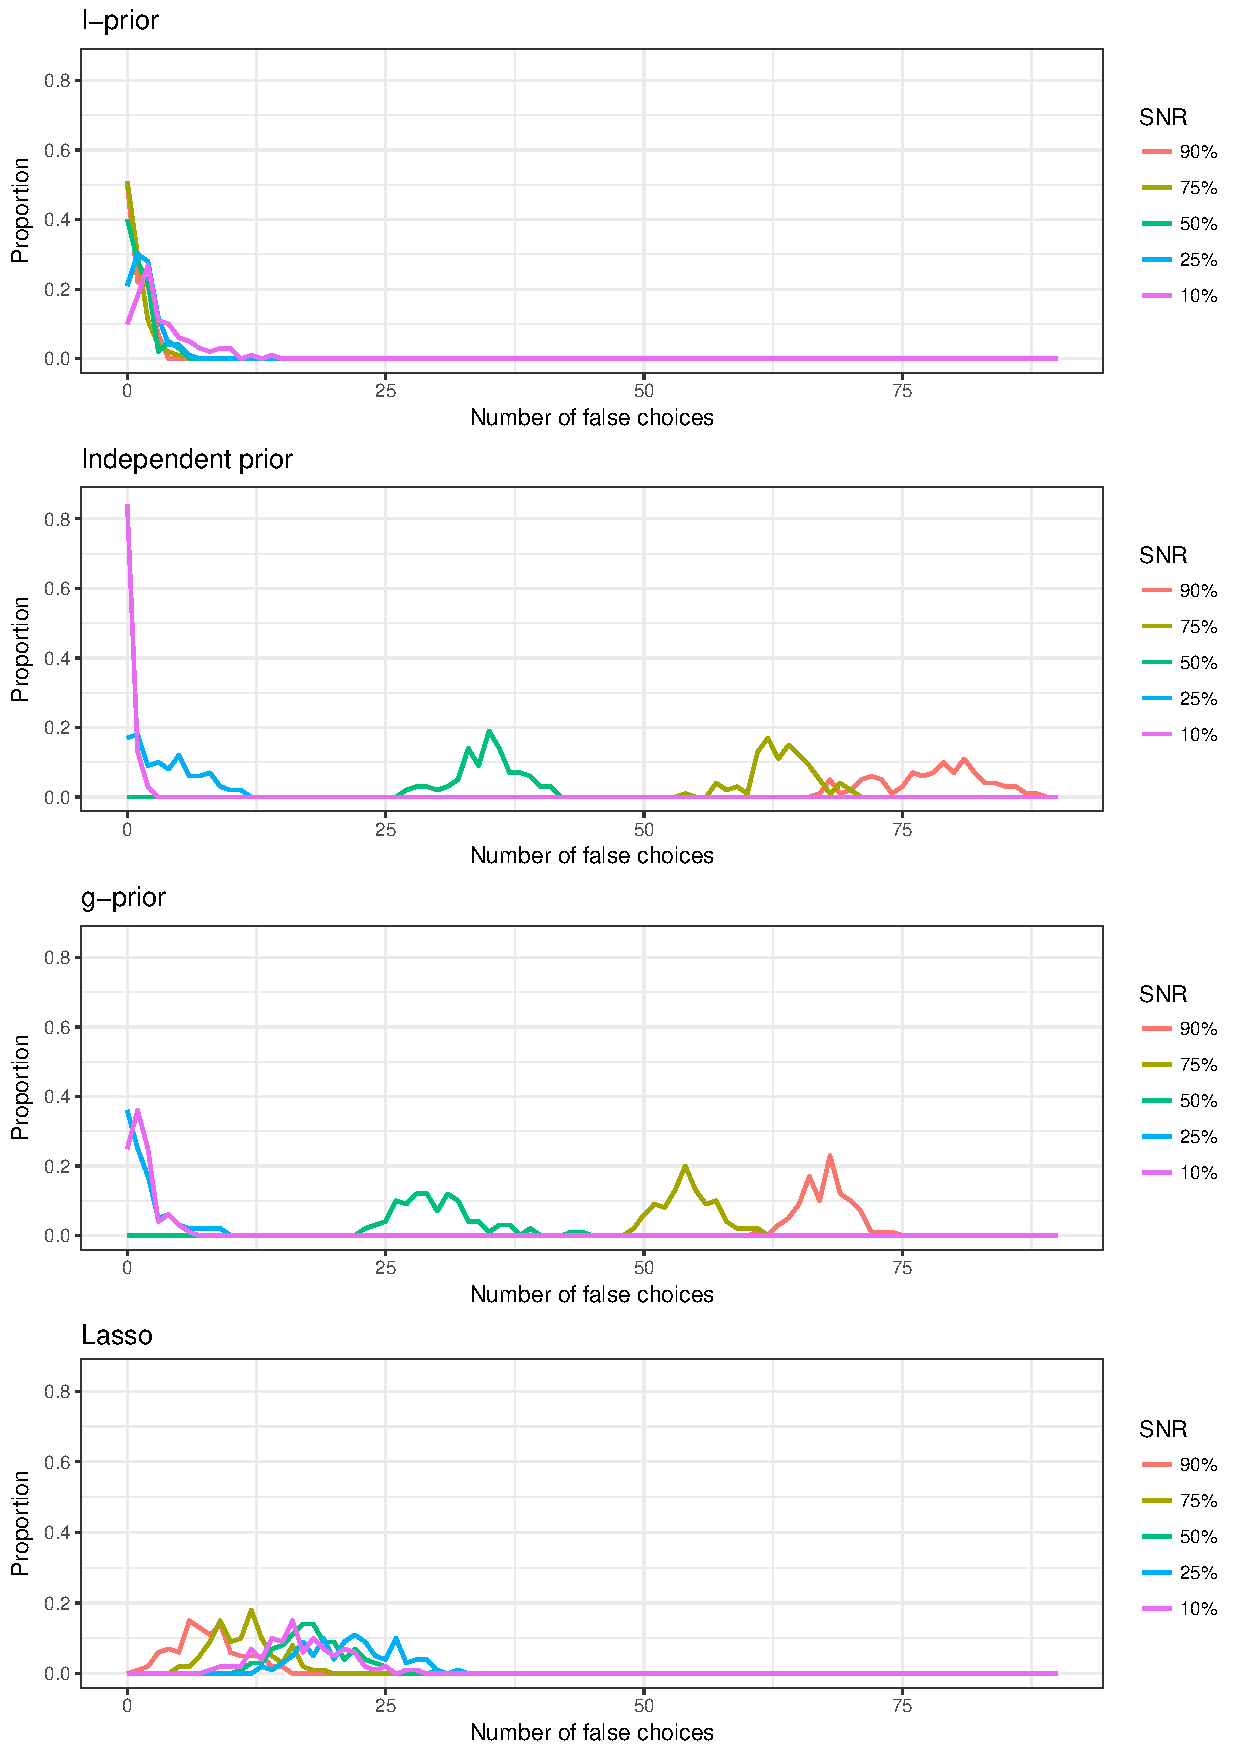
\includegraphics[scale=0.68]{figure/bvs_simres}
  \vspace{-1mm}
  \caption{Frequency polygons for the number of false choices for each of the four priors.}
  \label{fig:simres}
\end{figure}

\section{Examples}

Now, we apply our I-prior Bayesian variable selection model to three real-world data sets that have all been previously analysed in the variable selection literature.
In all analyses, a two-stage procedure was conducted for the I-prior model, where each stage consists of obtaining 15,000 MCMC samples (including 5,000 for burn-in).

\subsection{Aerobic data set}

This dataset appeared in the \textit{SAS/STAT\textsuperscript{\textregistered} User's Guide} \citep{SAS2008} and was also analysed by \citet{Kuo1998}. 
It involves understanding the factors which affect aerobic fitness, which is measured by the ability to consume oxygen. 
A sample of $n=30$ male participants' had their physical fitness measured by means of simple exercise tests. 
The response variable contains measurement of oxygen uptake rate in mL/kg body weight per minute. 
The six covariates were the participants' age ($X_1$), weight ($X_2$), time taken to run one mile ($X_3$), resting heart rate ($X_4$), heart rate while running ($X_5$), and maximum heart rate during the exercise ($X_6$). 
This dataset, although small in size, is interesting to analyse because of the correlations between the variables, mainly due to the measurements being taken during the same exercise test. 
Results are summarised in \cref{tab:aerobic}.
The sample correlations of interest are shown in Figure \ref{fig:aerobic-cor} below:

\begin{figure}[htb]
	\centering
	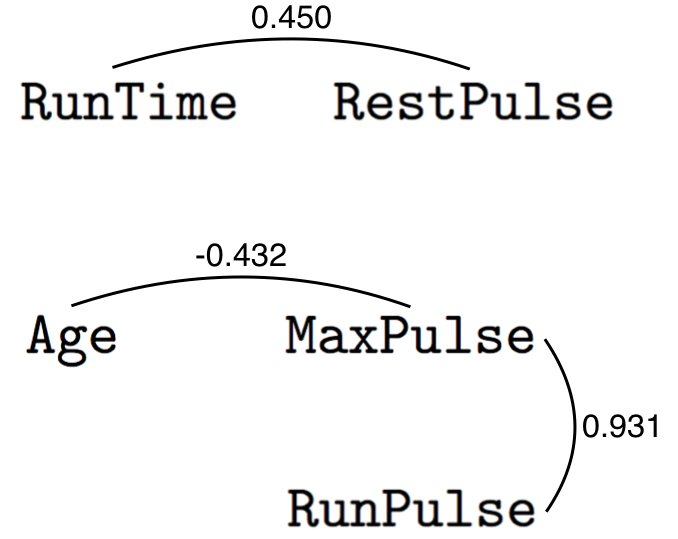
\includegraphics[height=1.3in]{figure/aerobic-cor}
	\caption{The sample correlations of interest in the aerobic fitness dataset. These show variables with correlations greater than 0.4 in magnitude. \label{fig:aerobic-cor}}
\end{figure}

\begin{table}[htb]
\centering
\caption{Results for variable selection of the Aerobic data set.}
\label{tab:aerobic}
\begin{tabular}{lrrrrr}
\toprule
      &PIP   &Model 1 &Model 2 &Model 3 &Model 4 \\
\midrule
$X_1$ &0.669 &\cmark  &        &\cmark  & \\
$X_2$ \\
$X_3$ &1.000 &\cmark  &\cmark  &\cmark  &\cmark \\
$X_4$ \\
$X_5$ &0.659 &\cmark  &        &        &\cmark \\
$X_6$ \\
\midrule
      &PMP   &0.564   &0.235   &0.105   &0.096 \\
      &BF    &1.000   &0.418   &0.187   &0.170 \\
\bottomrule
\end{tabular}
\end{table}

The highest posterior model selected was the model with the variables $X_1$, $X_3$ and $X_5$.
In \cref{fig:aerobic-densplot}, we can see that the point mass at zero overwhelms the rest of the values in the density plots for $X_2$, $X_4$ and $X_6$, and hence these variables were dropped.

\begin{figure}[H]
  \centering
  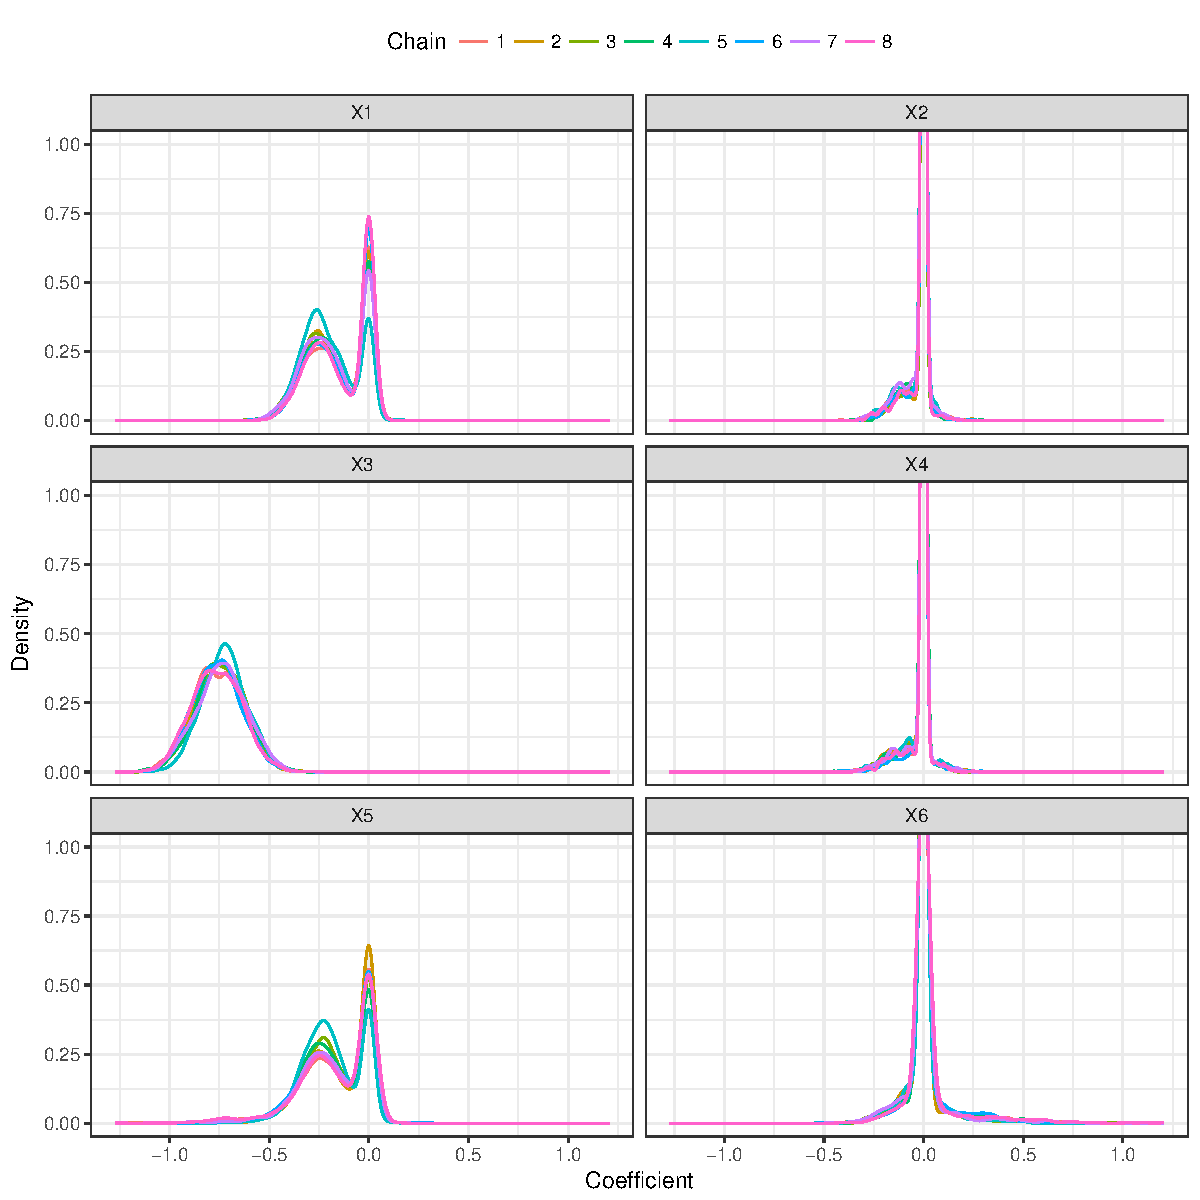
\includegraphics[width=\textwidth]{figure/aerobic_coef}
  \caption[Posterior density plots of the regression coefficients for the aerobic data set.]{Posterior density plots of the regression coefficients $\btheta$ for the aerobic data set. The `spike' at zero observed in the density plots for $X_2$, $X_4$ and $X_6$ is indicative of these variable being dropped often in the posterior samples.}
  \label{fig:aerobic-densplot}
\end{figure}

\subsection{Mortality and air pollution data}
\label{sec:airpollution}

The next real world application comes from a paper by \citet{McDonald1973}. 
In it, the effects of air pollution on mortality in a US metropolitan area ($n=60$ and $p=15$) were studied. 
The response variable is the total age adjusted mortality rate, and the main pollution effects of interest were that of hydrocarbons (HC), oxides of nitrogen (NO\textsubscript{x}) and sulphur dioxide (SO\textsubscript{2}). 
Several other environmental and socioeconomic considerations were taken into account, otherwise the model may include unexplained variation caused by factors other than pollution. 
For example, a metropolitan area with a high proportion of the elderly should expect to have a higher mortality rate than one with a low proportion. 
All of the variables can be considered as continuous and real. 
A full description of the data can be found in \cref{apx:airpollution}. 

This dataset also contains several highly correlated variables which impedes a meaningful regression analysis. 
When the full model is fitted using ordinary least squares, none of the pollutant effects were found to be significant. 
Clearly, a variable selection method was required. 
\citeauthor{McDonald1973} used a ridge regression technique to determine which variables to select and eliminate ``unstable'' coefficients found from a trace analysis. 
In addition, the authors also looked at a variable elimination method based on total squared error via Mallow's $C_p$.
The results are summarised in \cref{tab:poll}.

\begin{table}[htbp]
\centering
\caption[Results for the mortality and air pollution BVS model.]{A comparison of the coefficient values obtained using ordinary least squares (full model), \citeauthor{McDonald1973}'s minimum $C_p$ and ridge analysis, and the I-prior. Standard errors/posterior standard deviations are given in parentheses. Values shaded grey in the column of the full model indicate regression coefficients not significant at the 10\% level.}
\label{tab:poll}
\begin{tabular}{lrrrr}
\toprule
& Full model & Min. $C_p$ & Ridge  & I-prior \\ \midrule
\emph{Environmental factors} \\
\hspace{0.5em} Precipitation            & 0.306 (0.14)                 & 0.247 (0.07)   & 0.230 (0.07)      & 0.254 (0.12)       \\
\hspace{0.5em} Relative humidity        & {\color{gray} 0.009 (0.10)}  &                &                   &         \\
\hspace{0.5em} January temperature      & {\color{gray} -0.318 (0.18)} & -0.164 (0.06)  & -0.172 (0.06)     & -0.195 (0.11)        \\
\hspace{0.5em} July temperature         & {\color{gray} -0.237 (0.15)} & -0.073 (0.07)  &                   &         \\
\\
\emph{Demographic factors} \\
\hspace{0.5em} Population density       & {\color{gray} 0.084 (0.09)}  &                & 0.091 (0.06)      &         \\
\hspace{0.5em} Household size & {\color{gray} -0.232 (0.15)} &                &                   &         \\
\hspace{0.5em} Education                & {\color{gray} -0.233 (0.16)} & -0.190 (0.06)  & -0.171 (0.07)     & -0.151 (0.12)        \\
\hspace{0.5em} Sound housing units   & {\color{gray} -0.052 (0.15)} &                &                   &         \\
\hspace{0.5em} Age >65 years     & {\color{gray} -0.213 (0.20)} &                &                   &         \\
\hspace{0.5em} Non-white             & 0.640 (0.19)                 & 0.481 (0.07)   & 0.462 (0.07)      &  0.517 (0.10)       \\
\hspace{0.5em} White collar          & {\color{gray} -0.014 (0.12)} &                &                   &         \\
\hspace{0.5em} Income <\$3,000         & {\color{gray} -0.009 (0.22)} &                &                   &         \\
\\
\emph{Pollution potential} \\
\hspace{0.5em} HC    & {\color{gray} -0.979 (0.72)} &                &                   &         \\
\hspace{0.5em} NO\textsubscript{x} & {\color{gray} 0.983 (0.75)}  &                &                   &         \\
\hspace{0.5em}  SO\textsubscript{2} & {\color{gray} 0.090 (0.15)}  & 0.255 (0.06)   & 0.232 (0.06)      &  0.302 (0.09)        \\
\midrule
Size                     & 15                           & 6              & 6                 & 5         \\
$R^2$                    & 0.764                        & 0.541          & 0.553             & 0.676        \\ \bottomrule
\end{tabular}
\end{table}

In this case, the I-prior BVS model concurred with the overall finding of \citet{McDonald1973}, in that SO\textsubscript{2} was found to be a significant contributing factor towards mortality rates, while the rest of the pollutants were not.
the I-prior BVS model also obtained a model with the largest $R^2$ and the smallest size.


\subsection{Ozone data set}
\label{sec:ozone}

In this section, we replicate the Bayesian variable selection analysis of the Ozone dataset done by \citet{Casella2006} which appeared initially in \citet{Breiman1985}, and also show how Bayesian variable selection can help select important interaction terms. 
The data consists of daily ozone readings and various meteorological quantities, and the aim was to see which of these quantities contributed to the ozone concentration. 
The variables are explained in \cref{apx:ozone}. 

The data contains 366 points, one for each day of the leap year 1976. 
There are 163 data points containing missing data on some of the predictors, so we did a complete case analysis on the remaining 203 samples. 
Out of these 203, we randomly set aside 25 to use for validation, thus the $n$ used to train the model was $n=178$. 
The training and test set were repeated multiple times and results averaged in order to make a comparison to the unknown training and test set used in the other studies.
Out-of-sample prediction root mean squared errors (RMSE) were obtained, as well as the coefficient of determination $R^2$.

\citeauthor{Casella2006} removed the variables $X_{11}$ and $X_{12}$ before running their selection model, citing multicollinearity causing ill-conditioned design matrices. 
Upon inspection, there are indeed correlations among the variables as high as 0.93 for some of them, but not enough to cause rank deficiency in the design matrix and a degenerate $\XTX$ matrix.
The correlations $\Corr(X_7,X_{11}) =0.91$ and $\Corr(X_{11},X_{12}) = 0.93$ seemed to drive the decision to drop the two variables, and while it is a valid concern, we will conduct variable selection on the full set of 12 variables.
We can then see the performance of I-priors in the presence of multicollinearity in this real-world data set. 
On another note, the variables $X_1$, $X_2$ and $X_3$ were presumably intended to be categorical as in modelling seasonality in a time series data, but these were treated as continuous, as did \citeauthor{Casella2006}. 
The results are compared in \cref{tab:ozoneres}.

\begin{table}[htb]
\centering
\caption{Results for variable selection of the Ozone data set using only linear predictors.}
\label{tab:ozoneres}
\begin{tabular}{llrrrr}
\toprule
Method                          &Variables            &Size &$R^2$ &RMSE \\
\midrule
I-prior                         &$X_1,X_6,X_{11}$     &3    &0.708 &0.554 \\
\citeauthor{Casella2006} (C\&M) &$X_6,X_7,X_8$        &3    &0.686 &0.992 \\
\citeauthor{Breiman1985} (B\&F) &$X_7,X_8,X_9,X_{10}$ &4    &0.669 &1.056 \\
\bottomrule
\end{tabular}
\end{table}

What we found was that the model selected using the I-prior does better in terms of $R^2$ as well as RMSE compared to the methods used by C\&M and B\&F. 
The average posterior model probability for $X_1,X_6,X_{11}$ as found by the I-prior was 0.722\footnotemark. 
One thing to note is that the I-prior model selected the variable $X_{11}$ instead of its highly correlated proxy $X_7$, which is what C\&M selected.
These two variables are temperature measurements at different locations in California.
As C\&M excluded $X_{11}$ from the model search it was of course never considered in their model selection process, and because we included it in ours, the variable selection method was able to consider both variables together and decide on the more appropriate one. 
Unless there is a strong insistence on deleting variables beforehand, we might not know for sure whether the variable was rightfully removed from consideration, as this example seems to prove.
Out of interest, running the variable selection model on the reduced variable space as C\&M did, we arrive at the same results as theirs.

\footnotetext{Since the total model space used was different between our method, C\&M and B\&F, it does not make sense to compare posterior model probabilities which we obtained. C\&M reported a model probability of 0.491 for their model, but this model was not selected at all using the I-prior.}

We then used the I-prior method to select between the squared terms and all level two interactions, in addition to all the variables, in an effort to improve model prediction. 
For 12 such variables, the number of variables to select becomes $12 + 12 + 12(12 - 1)/2 = 90$. 
By doing so, we were able to improve the model to give a slightly better predictive ability.
The results are shown below in \cref{tab:resozone2}. 
The I-prior again selected a model which was superior in terms of $R^2$ and RMSE compared to that obtained by C\&M.

\begin{table}[htb]
\centering
\caption{Results for variable selection of the Ozone data set using linear, squared and two-way interaction terms.}
\label{tab:resozone2}
\begin{tabular}{llrrrr}
\toprule
Method                          &Variables            &Size &$R^2$ &RMSE \\
\midrule
I-prior                         
&{\footnotesize $X_1,X_5,X_6,X_{11},X_{12},X_1^2,X_9^2,X_6X_{11},X_6X_{12},X_7X_9$}     
&10    &0.812 &0.503 \\
C\&M
&{\footnotesize $X_2,X_1^2,X_7^2,X_9^2,X_1X_5,X_2X_6,X_3X_7,X_4X_6,X_6X_8,X_6X_{10}$}   &10    &0.758 &0.873 \\
\bottomrule
\end{tabular}
\end{table}

\section{Conclusion}

The Bayesian variable selection methods that we have seen have the appeal of reducing the problem of model search into one of estimation. 
At the outset, we aimed to seek a model which: 1) requires little tuning on the part of the user; 2) would work well in the presence of multicollinearity; and 3) is able to work well with little to no prior information. 
The I-prior on the regression coefficients in \citeauthor{Kuo1998}'s spike-and-slab stochastic search framework achieves this aim.

The attractive feature about the Bayesian approach to variable selection is the ability to simultaneously shrink and select predictors, thereby incorporating model uncertainty in the regressors.
Sparsification is not ``hard coded'', in the sense that variables are assigned a value of zero with some positive probability in the posterior.
This is unlike the regularisation or penalised log-likelihood approach to variable selection using the Lasso, elastic net, and so on, whereby sparsity is induced at the mode, but not in the posterior distribution \citep{scott2014predicting}.
This translates to being provided with a single variable selection decision, rather than information that is coded through a probability distribution.

We discuss three areas to concentrate on for future research and improvement:
\begin{enumerate}
  \item \textbf{\boldmath$p>n$ cases}. 
  Typically, when there is insufficient information in the data to inform the estimation, then additional information is sought from the priors. 
  In our case, the I-prior covariance involves the inverse of a low rank matrix which is not invertible.
  A $p$-variate normal distribution with a singular covariance matrix will only have a probability distribution defined on a low dimensional subspace.
  The issue may however be computational---it might be worth exploring the generalised inverse, or study ways in which to avoid the inverse computation in the Gibbs sampler.
  
  \item \textbf{Improvement in computational time}. 
  Although the model itself is not computationally intensive to run (roughly $O(np^2)$ in time per Gibbs iteration), the main bottleneck is the reliance on a stochastic sampling algorithm.
  As in the previous chapter, variational inference is a promising area to look into, especially given that the Gibbs conditional distributions were straightforward to obtain, and these might be similar to a mean-field variational distribution.
  If this is successful, then it is expected to reduce computational time and avoid convergence issues that comes with traditional MCMCs.
  
  \item \textbf{Extension to generalised linear models}.
  \citet{Kuo1998} in their paper already provided a sketch of how the variable selection model would work.
  In our case, it would also require careful consideration of the appropriate covariance matrix for the regressors, to keep in line with the definition of I-priors.
\end{enumerate}

Finally, it should be mentioned that more complex variable selection models can be coded with the $\gamma$ indicators.
For instance, in selecting squared or interaction terms, we can insist on having the model select the main term if the squared or interaction term is selected:
\[
  y_i = \alpha + \max(\gamma_1,\gamma_3) \beta_1x_{1i} + \max(\gamma_1,\gamma_3) \beta_2 x_{2i} + \gamma_3 \beta_3 x_{1i}x_{2i}.
\]
Or perhaps, we could use a single $\gamma$ indicator for the dummy variables which make up a single categorical covariate, which we would then infer on the selection of the single covariate rather than each individual category of the covariate.

%\section{Miscellanea}
%\subsection{Recap: Bayesian linear regression}

The ordinary least squares (OLS) estimates for the $\beta$ coefficients is given by $\hat\beta = (X^\top X)^{-1} X^\top y$, where $y$ is the $n$-vector of responses.
This is obtained by maximising the normal likelihood of $\beta$, but interestingly, the exact same solution is obtained by minimising the sum of squared errors - without having to set any distributional assumption on the errors. 
Thus the form of the solution comes from only what is known to us: the data, $X$ and $y$.

The Bayesian approach to estimating the linear model takes a different outlook, in that it supplements what is already known from the data with additional information in the form of prior beliefs about the parameters $\Theta$, or simply, priors. 
Inferences about the parameters are then performed on the posterior
\[
  p(\Theta|y) \propto 
  {\color{gray} \overbrace{\color{black} p(y|\Theta)}^{\text{likelihood}}} 
  \times 
  {\color{gray} \overbrace{\color{black} p(\Theta)}^{\text{prior}}}
\]
such as taking the mean, which is known as the Minimum Mean Squared Error estimate (MMSE), or the mode, which corresponds to the maximum a posteriori estimate (MAP).
The Bayesian approach of MAP is similar to maximum likelihood, but differs only in the fact that the optimisation objective (the likelihood function) is augmented with a prior distribution about the parameters. 

For the normal linear model \eqref{eq:linmod}, conjugate priors for the regression coefficients of the form
\[
  \beta | \sigma^2 \sim \N(b, \sigma^2 B) 
\]
are popular, which results in the normal posterior distribution for $\beta$ with mean and variance
\[
  \tilde b = (X^\top X + B^{-1})^{-1}(X^\top y + B^{-1}b) \hspace{0.5cm}\text{and}\hspace{0.5cm} \tilde B = (X^\top X + B^{-1})^{-1}
\]
respectively.
The choice of the prior hyperparameters $b$ and $B$ reflects one's belief about prior knowledge surrounding the parameters to be estimated.
For the prior mean, $b = 0$ is a reasonable and convenient choice after standardising the data, since scaling and centring the data does not affect the validity of the model.
Further, setting $B = \lambda I_p$, where $I_p$ is the identity matrix, is also common practice.
Large values of $\lambda$ may be chosen to reflect the uninformativeness of the prior distribution.
In this setting, the posterior solution for $\beta$ resembles that of \emph{ridge regression}.

Another type of prior that is popular for linear regression (and in fact in variable selection too) is the $g$-prior \citep{zellner1986assessing}: $\beta \sim \N(0, \sigma^2 g (X^\top X)^{-1})$.
The $g$-prior has the very convenient property of reducing the posterior and marginal distributions of the linear model to formulae involving the OLS estimator $\hat\beta$, the residual sum of squares $\Vert y - X\hat\beta \Vert^2$, and the hyperparamater $g$ \citep{fernandez2001benchmark}.
Many studies have delved into appropriate choices or estimation procedures for $g$ \citep{liang2008mixtures}.

On the topic of variable selection, the Lasso \citep{tibshirani1996regression} is a popular deterministic method which has the unique property that the L-1 penalised least squares solution for the regression coefficients may be exactly zero for some of them.
Some may view the L-1 penalty as having a Bayesian interpretation, in that double exponential or Laplace priors are placed on the $\beta$ \citep{park2008bayesian}.



\hClosingStuffStandalone
\end{document}